\section*{Blur: Experimentación}

Antes de comenzar con la experimentación supusimos que ambas implementaciones iban a ser más rápidas que las de C, las razones serán explicadas más adelante. Sin embargo, no estamos seguros de que versión de assembler tendrá mejor desempeño.
Esto se debe a que ambas tienen sus pros y sus contras. Por ejemplo, la segunda versión, aunque levanta de a más píxeles, es más compleja y tiene 2 saltos condicionales, mientras que la primera versión levanta de a menos pixeles, mientras que el cálculo es más simple. Por lo visto en clase, suponemos que pesa mas el hecho de tener un mejor patrón de acceso a memoria.

Justamente lo interesante de este filtro es que nos permitirá definir qué pesa mas a la hora de la performance, si un buen patrón de accesos a memoria o cálculos simples. Aunque ambos aspectos son muy importantes, es interesante saber cual pesa mas a la hora de hacer optimización mas fina de nuestros programas.

\begin{figure}[!hbt] 
	\centering
  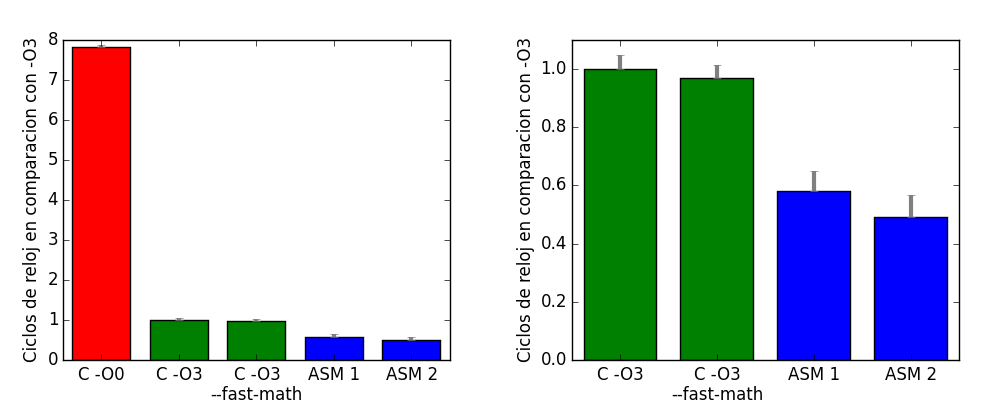
\includegraphics[width=20cm]{blur-all.png}
  \caption{Comparación de la cantidad de ciclos de reloj utilizada por diferentes variantes de merge. Para tener una medida absoluta: la cantidad de ciclos de reloj promedio de C -O3 es 4,292,457. Tamaño de la muestra: 200 imagenes de $16 \times 10^4$ píxeles. Se indica el mínimo con la barra y el promedio con una linea gris.}
\end{figure}

Como se puede ver en los resultados, nuestras hipótesis sobre el desempeño de assembler contra el desempeño de C eran correctas, la performance es superior. Sin embargo, la performance de las dos versiones de assembler son muy similares. Analizaremos esto mas adelante.


En general, para imagenes de tamaños standard, todas las implementaciones escalan linealmente, la única diferencia radica en la pendiente de las funciones, las de C tienen pendiente mucho mayor a las de assembler. El desempeño no depende de la imagen, dado que el tratamiento que se le hace a cada pixel no depende para nada de su contenido.
\\

Una posible mejora para el código propuesto (y aplica también para merge y hsl) es la utilización de registros AVX, que nos proveen del doble de capacidad, ya que podríamos levantar de a más pixeles, reduciendo ampliamente los accesos a memoria.
Otra posible mejora para las implementaciones de blur, se podría tener solo un loop en vez de dos como tiene nuestra implementación (para filas y para columnas). Esto ahorraría algunos saltos condicionales, que pueden llegar a causar problemas por branch mispredictions.
Sin embargo, esta alternativa es de más difícil implementación y realmente no estabamos 100\% seguros de que signifique una mejora importante.
\\

La función de C realiza mas accesos a memoria que las funciones de assembler. Esto se debe a que analiza cada canal del pixel por separado, en vez de todos juntos como nuestras implementaciones. Esto significa el triple de accesos a memoria, que claramente se ve reflejado en una pérdida de performance.

Los patrones de acceso a memoria de las dos implementaciones de assembler son bastante distintos. La primera implementación tiene más accesos, mientras que la segunda tiene menos, a costo de mayor complejidad en el código. Sin embargo, la diferencia no es drástica, ya que la segunda implementacion, cada 4 pixeles hay 3 lecturas a memoria, mientras que en la primera implementación hay 4 lecturas. La diferencia no es drástica, aunque asintoticamente puede ser que se refleje en una pendiente un poco mas baja de la segunda implementación.

Otro problema en cuanto a la memoria es el acceso alineado a las constantes que se usan a lo largo del programa (por ejemplo, la constante 9.0 que debemos usar para dividir). Sin embargo, como este problema es más profundo en el filtro de HSL, será analizado allí con la debida profundidad.
\\

Los saltos condicionales en ambas implementaciónes son algo que debemos analizar. Si una imagen tiene $n$ pixeles de ancho y $m$ de alto, entonces ambos algoritmos estarán frente una cantidad de saltos condicionales del orden de $nm+m$.
Esto no es realmente problemático, dado que como mínimo debemos realizar $nm$ saltos condicionales, y cambiar el código a esa alternativa requeriría más lógica y mas complejidad que revertirían lo positivo de ahorrar saltos.
\\

En cuanto al error generado por nuestras implementaciones, es fácilmente chequeable que es despreciable. Esto se debe principalmente a que el algoritmo es básicamente el mismo que el de C, es decir, usamos números de punto flotante y hacemos lo mismo que el programa de C, solo que más eficientemente.













